\begin{frame}
  \centering
  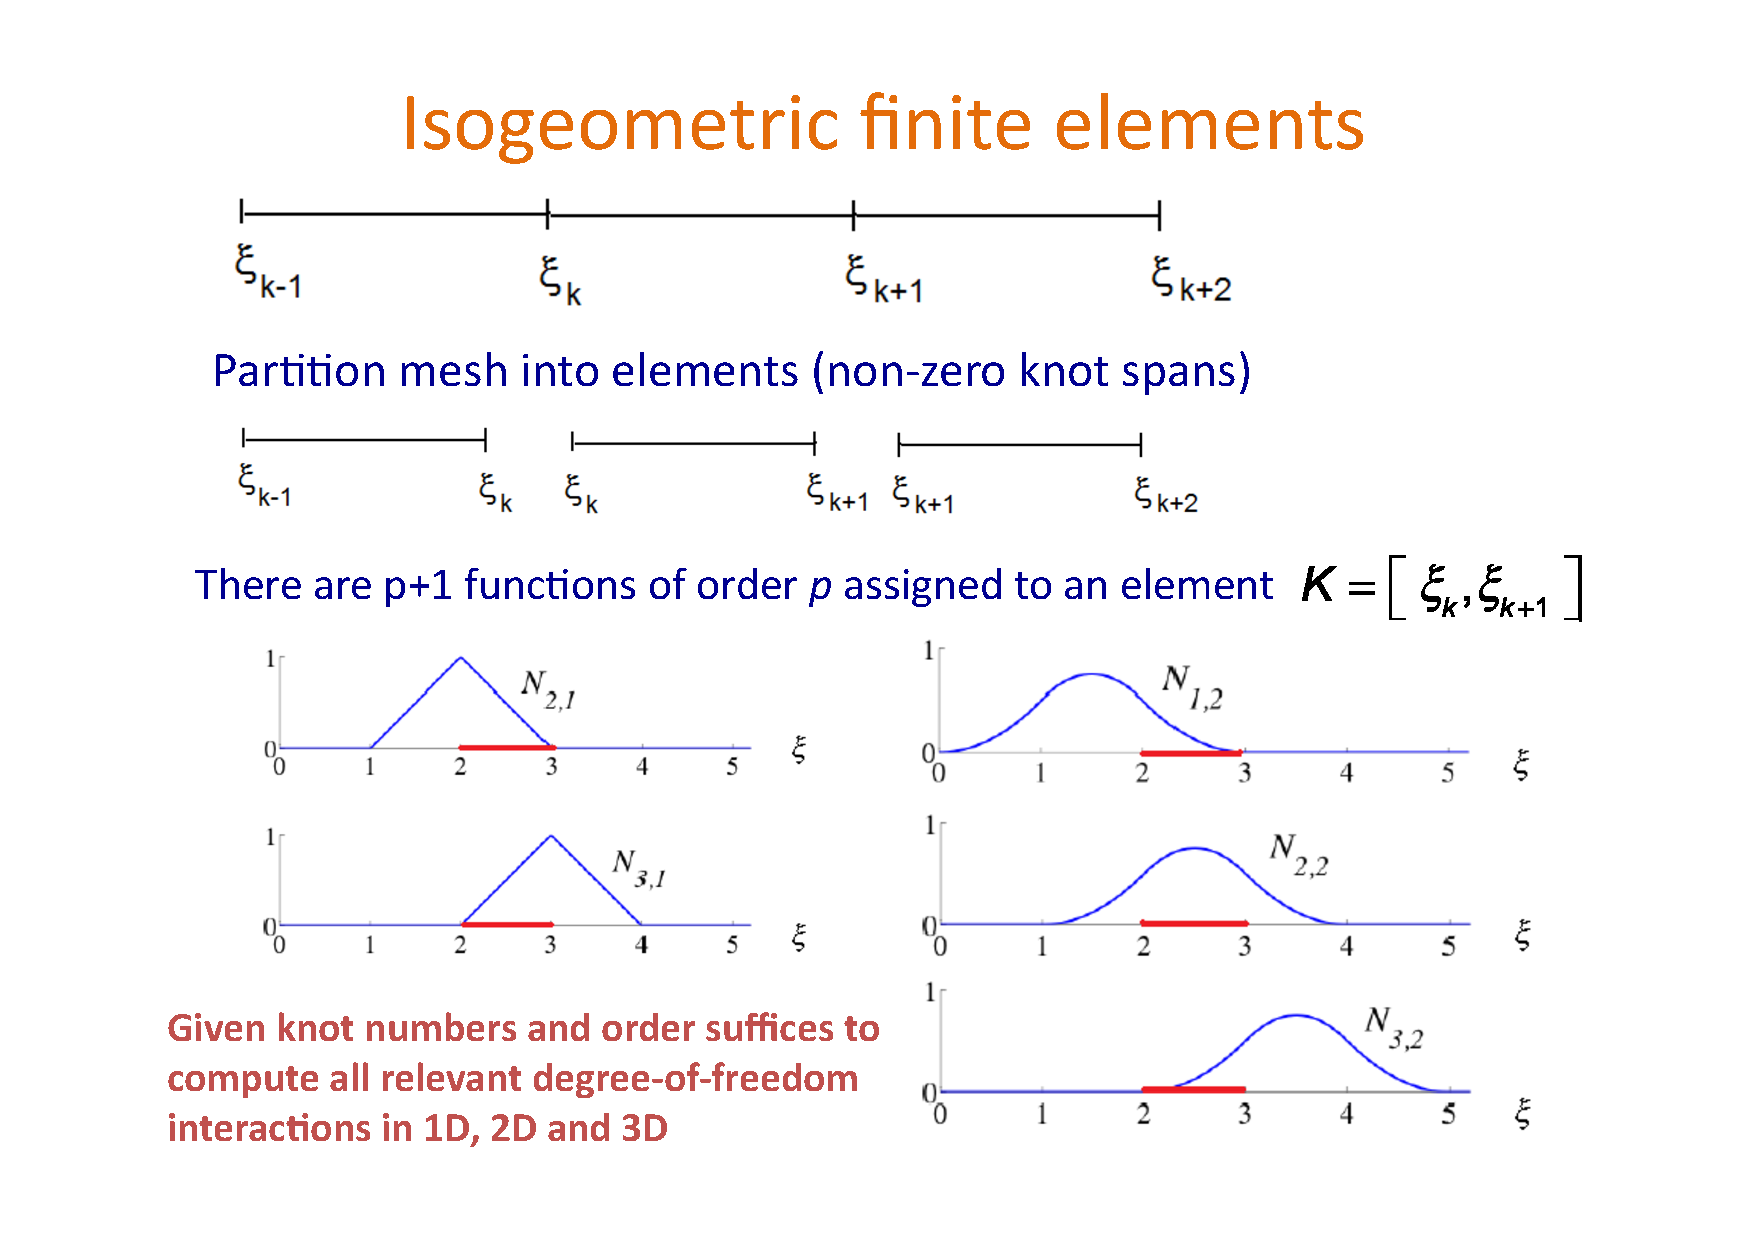
\includegraphics[width=1.1\textwidth]{figures/IGACalo}
%  (c/o Victor Calo)
\end{frame}

\begin{frame}{IGA compared to standard FEM}
  \begin{itemize}
  \item Can exactly conform to some engineering geometries.
  \item Better impedence match with solid modeling (CAD).
  \item Fewer degrees of freedom for 4th order problems,\\
    \quad \eg no rotation dofs for shells.
  \item More nonzeros per row as continuity is increased.
  \item More quadrature points per dof (higher arithmetic intensity).
  \item Needs logically structured grids \\
    (T-splines can join structured patches)
  \item All-positive basis functions useful for some problems \\
    (maintain positivity, robust conservative normals)
  \item Non-interpolatary basis can be tricky for preconditioning.
  \end{itemize}
\end{frame}

\begin{frame}
  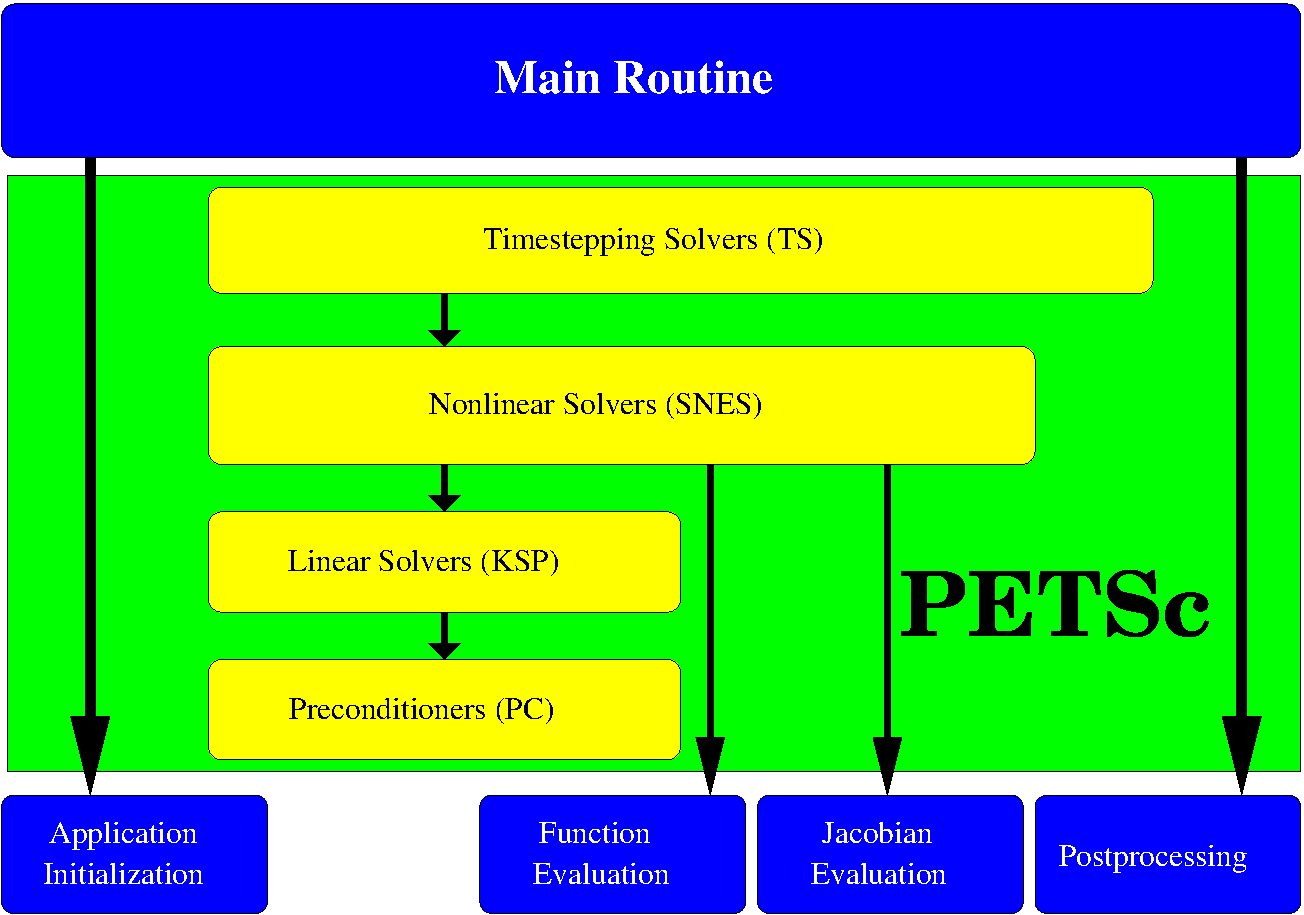
\includegraphics[width=0.8\textwidth]{figures/SNES/FlowControl}
  \begin{itemize}
  \item IGA used to evaluate nonlinear residuals
  \item PETSc \cverb|DA| used to manage parallelism.
  \item Adaptive time integration using method of lines.
    \begin{itemize}
    \item Generalized $\alpha$ method from PETSc \cverb|TS|.
    \end{itemize}
  \item Matrix-free Newton-Krylov, need only residuals for implicit solve.
  \end{itemize}
\end{frame}

% \begin{frame}{Cahn-Hilliard Equation}
%   Models phase separation: find concentration $c$
%   \begin{equation*}
%     \ip{w}{\frac{\partial c}{\partial t}}_\Omega + \ip{\nabla w}{M(c)\nabla\mu(c) + \nabla M(c)\Delta c}_\Omega + \ip{\Delta w}{M(c) \Delta c}_\Omega = 0 \quad \forall w
%   \end{equation*}
%   Boundary conditions and equations of state $\mu(c)$ and $M(c)$.
%   \begin{minted}[gobble=4]{c}
%     R_rho  = Na*rho_t;
%     R_rho += -rho*(Na_x*ux + Na_y*uy);

%     R_ux  = Na*ux*rho_t;
%     R_ux += Na*rho*ux_t;
%     R_ux += -rho*(Na_x*ux*ux + Na_y*ux*uy);
%     R_ux += -Na_x*p;
%     R_ux += rRe*(Na_x*tau_xx + Na_y*tau_xy);
%     R_ux += -Ca2*rho*(Na_xx*rho_x + Na_xy*rho_y);
%     R_ux += -Ca2*Na_x*(rho_x*rho_x + rho_y*rho_y);
%     R_ux += -Ca2*Na*(rho_xx*rho_x + rho_xy*rho_y);
%     R_ux += -Ca2*rho_x*(Na_x*rho_x + Na_y*rho_y);
%   \end{minted}
% \end{frame}

\begin{frame}[fragile,shrink=5]{Navier-Stokes Korteweg}
  Phase field model for water/water vapor two-phase flows.
  Find $U = (\rho,\uu)$ such that $B(W,U) = 0$ for all $W = (q,\ww)$, plus boundary conditions.
  \begin{equation*}
    \begin{split}
      B(W,U) &= \int_\Omega q \frac{\partial \rho}{\partial t} - \nabla q\cdot \rho\uu
      + w\cdot \left[\uu\frac{\partial\rho}{\partial t} + \rho\frac{\partial \uu}{\partial t} \right] \\
      &+ \nabla w \tcolon \Big[ -\rho\uu\otimes\uu + \tau - (p + \lambda \abs{\nabla \rho}^2)\bm 1 \Big] \\
      &- \nabla(\nabla\cdot\ww)\cdot \lambda\rho\nabla\rho - \nabla(\nabla\rho\cdot\ww)\cdot\lambda\nabla\rho = 0
    \end{split}
  \end{equation*}
  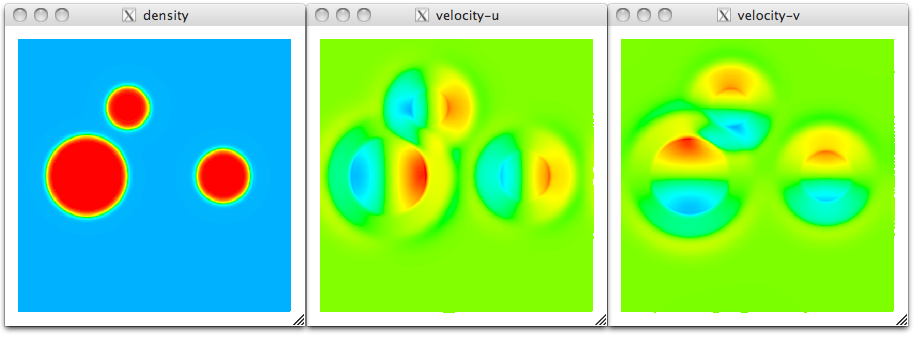
\includegraphics[width=\textwidth]{figures/NSK}
\end{frame}

\begin{frame}[fragile,shrink=5]{Navier-Stokes Korteweg}
  Phase field model for water/water vapor two-phase flows.
  Find $U = (\rho,\uu)$ such that $B(W,U) = 0$ for all $W = (q,\ww)$, plus boundary conditions.
  \begin{equation*}
    \begin{split}
      B(W,U) &= \int_\Omega q \frac{\partial \rho}{\partial t} - \nabla q\cdot \rho\uu
      + w\cdot \left[\uu\frac{\partial\rho}{\partial t} + \rho\frac{\partial \uu}{\partial t} \right] \\
      &+ \nabla w \tcolon \Big[ -\rho\uu\otimes\uu + \tau - (p + \lambda \abs{\nabla \rho}^2))\bm 1 \Big] \\
      &- \nabla(\nabla\cdot\ww)\cdot \lambda\rho\nabla\rho - \nabla(\nabla\rho\cdot\ww)\cdot\lambda\nabla\rho = 0
    \end{split}
  \end{equation*}
  \begin{minted}[gobble=2]{c}
  for each Na,Na_x,Na_xx,Na_y,Na_yy: // test functions
    R_rho  = Na*rho_t;
    R_rho += -rho*(Na_x*ux + Na_y*uy);
    R_ux  = Na*ux*rho_t;
    R_ux += Na*rho*ux_t;
    R_ux += -rho*(Na_x*ux*ux + Na_y*ux*uy);
    R_ux += -Na_x*p;
    R_ux += rRe*(Na_x*tau_xx + Na_y*tau_xy);
    R_ux += -Ca2*rho*(Na_xx*rho_x + Na_xy*rho_y);
    ...
  \end{minted}
\end{frame}

\begin{frame}[fragile]{Transform to more vector-friendly form}
  \begin{itemize}
  \item Pre-compute ``physics'' \cverb|W| at each quadrature point
  \item assembling the residual becomes dot products
  \begin{minted}[gobble=2]{c}
  for each Na,Na_x,Na_xx,Na_y,Na_yy:
    R_rho  = Na*W[irho_t];
    R_rho += Na_x*W[rho_nax];
    R_rho += Na_y*W[rho_nay];
    R_ux  = Na*W[ux_na];
    R_ux += Na_x*W[ux_nax];
    R_ux += Na_y*W[ux_nay];
    R_ux += Na_xx*W[u_naxx];
    R_ux += Na_xy*W[u_naxy];
  \end{minted}
  \item 1.9x speedup
  \end{itemize}
\end{frame}

\begin{frame}[fragile]{Vectorize using SimASM}
  \begin{itemize}
  \item Define context-sensitive vector primitives
    \begin{minted}[gobble=4]{python}
      def muladd_copy(self, com, rt, ra, rb):
        if ra[1] == 0:
          return isa.fxcpmadd(rt,com.W[ra[0]],rb,rt)
        else:
          return isa.fxcsmadd(rt,com.W[ra[0]],rb,rt)
    \end{minted}
  \item Unrolled/jammed vector assembly looks ``close'' to the physics
    \begin{minted}[gobble=4]{python}
      [self.muladd_copy(com, 'R_rho', com.rho_nax, 'Na_x'),
      self.muladd_copy(com, 'R_ux', com.ux_nax, 'Na_x'),
      self.muladd_copy(com, 'R_uy', com.uy_nax, 'Na_x')]
    \end{minted}
  \item Still limited by load/store unit.
  \item Multiple quadrature points and elements could amortize load/store cost.
  \item More clever transformations?
  \item Still need to optimize computation of coordinate transformation for high end-to-end throughput.
  \end{itemize}
\end{frame}
